% Onpersoonlijk:
\section{Wat zijn de belangrijke aspecten van de kavels VI en VII?} \label{Wat zijn de belangrijke aspecten van de Kavels VI en VII?}

Er zijn veel aspecten van de kavels VI en VII waar rekening mee moet worden gehouden. Enkele belangrijker dan anderen. Ten eerste is de locatie van de kavels van belang. De kavels maken onderdeel uit van het windenergiegebied Hollandse Kust west en liggen op ongeveer 53 km van de west kust van Nederland en heeft een oppervlakte van circa 176 km\textsuperscript{2}.\cite{SiteDescriptionRVO} De twee kavels zullen elk een \gls{offshore} windcapaciteit van 700MW realiseren.\cite{SiteDescriptionRVO}\cite{Functies&gebruikHKW}

Om het windpark te ontwerpen dat instaat is dit te bieden zijn verschillende andere data van de kavels belangrijk. Er moet bepaald worden wat de beste positionering is voor de windturbines. Bij de beslissing hiervan moeten aspecten in acht genomen worden, zoals al bestaande en geplande infrastructuur van pijpleidingen en kabels. Daarnaast moet rekening worden gehouden met potentiële wrakken, magnetische abnormaliteiten en oude boorgaten zoals genoteerd staat in Appendix C van de locatie beschrijving (zie figuur \ref{fig:obstakels}).\cite{SiteDescriptionRVO}\cite{AppendixC} Uit voorzorg zullen, de windturbines op een minimale afstand van 100 meter van de genoemde obstakels geplaatst worden. Dit zal echter pas later van toepassing zijn, aangezien er voorlopig nog geen parkindeling is gemaakt. 
\begin{figure}[h]
\centering
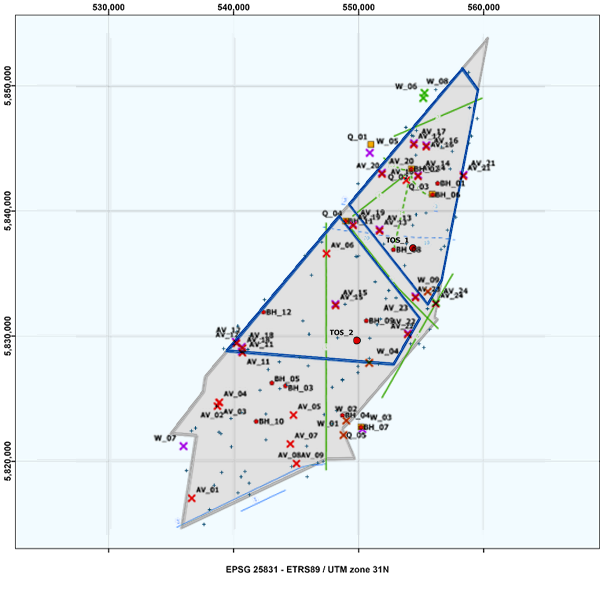
\includegraphics[width=0.5\textwidth]{IMG/data/overzicht/Map.png}
\caption{Gecombineerde map van obstakels.}
\label{fig:obstakels}
\end{figure}

Er is ook informatie over de kavels die significant is voor het besluit over de te kiezen windturbines en de oriëntatie hiervan. De informatie die hiervoor belangrijk is, is de winddata, zoals windsnelheden en -richtingen over langere periodes. Deze data is te halen uit de Wind Resource Assessment.\cite{WindResourceAssessment} In dit document staat winddata van metingen die zijn uitgevoerd over een periode van twee jaar, van 07-02-2019 tot 06-02-2021. Deze metingen zijn gedaan op een hoogte van 100 meter boven het gemiddelde zeeniveau en zijn dus representatief voor de te verwachten winden die de windturbines zullen ervaren. De statisch gemiddelde gemeten windsnelheid was over deze periode 10,06 m/s. 

Behalve de windsnelheid, is ook de windrichting van belang. De windrichting was net zoals de windsnelheid variërend, echter is er wel een overheersende windrichting bepaald. De overheersende windrichting is WZW (West-Zuid-West), deze windrichting kwam voor 21,2\% van de gemeten periode voor. De tweede meest significante windrichting was ZZW (Zuid-Zuid-West), met 20,1\%. 





% Er is naar een veelvoud windturbines gezocht en gekeken. Bekeken modellen waren onder andere de volgende:
% \begin{itemize}
%     \item De SG 14-236 DD, 14 MW windturbine van Siemens Gamesa.\cite{SiemensGamesa14MW}
%     \item De V236-15.0, 15 MW windturbine van Vestas.
%     \item De Haliade-X, 12 MW windturbine van GE renewable energy.\cite{GEHalideX}
%     \item 
% \end{itemize}

\section{Berekeningen}
\subsection{Algemene berekeningen}
\subsubsection{Swept Area}
Van de uitgekozen windturbines zijn meerdere gegevens verzameld, waaronder de diameter. Hiermee is het rotoroppervlakte (A(\(m^2\))) te berekenen zoals gedaan in formules \ref{eq:1} en \ref{eq:2}.
\begin{equation} \label{eq:1}
% \text{12MW Turbine geeft: } \pi*(\slashcirc/2)^2 = \pi*(222/2)^2 = 38707
\text{12MW Turbine geeft: } A =\pi*(\frac{\slashcirc_{12MW}}{2})^2 = \pi*(\frac{222}{2})^2 = 38707 m^2
\end{equation}
\myequations{Berekening: A 12MW Turbine}

\begin{equation} \label{eq:2}
\text{18MW Turbine geeft: } A =\pi*(\frac{\slashcirc_{18MW}}{2})^2 = \pi*(\frac{263}{2})^2 = 54325 m^2
\end{equation}
\myequations{Berekening: A 18MW Turbine}

De diameter van de twee turbines verschilt, vanwege de kwadratische berekening die gepaard gaat met het berekenen van de oppervlakte, is het effect hiervan groter terug te zien in het rotoroppervlak.
\subsubsection{Theoretisch vermogen}
Met het rotoroppervlak van de turbines is het theoretische vermogen dat uit de wind gehaald kan worden, te berekenen. Dit vermogen kan berekend worden met de formules \ref{eq:3} en \ref{eq:4} hieronder. 

\begin{equation} \label{eq:3}
    P_{wind12MW} = \frac{1}{2}*1.29*A_{12MW}*v_{wind}^3 = \frac{1}{2}*1.29*38707*v_{wind}^3
\end{equation}
\myequations{Berekening: Pwind 12MW Turbine}

\begin{equation} \label{eq:4}
    P_{wind18MW} = \frac{1}{2}*1.29*A_{18MW}*v_{wind}^3 = \frac{1}{2}*1.29*54325*v_{wind}^3
\end{equation}
\myequations{Berekening: Pwind 18MW Turbine}

\subsubsection{Tussenberekeningen}
De snelheid van de wind op de kavels is variërend, deze formules zijn dus toegepast voor realistische en te verwachten windsnelheden gebaseerd op de windgegevens over een periode van twee jaar.\cite{WindResourceAssessment} 
De uitkomsten zijn in een tabel genoteerd en geplot zoals te zien in (figuur \ref{fig:TVUW}). In realiteit is dit theoretische vermogen niet volledig uit de wind te halen, er is namelijk sprake van het Betzlimiet. 

\begin{figure}[H]
\centering
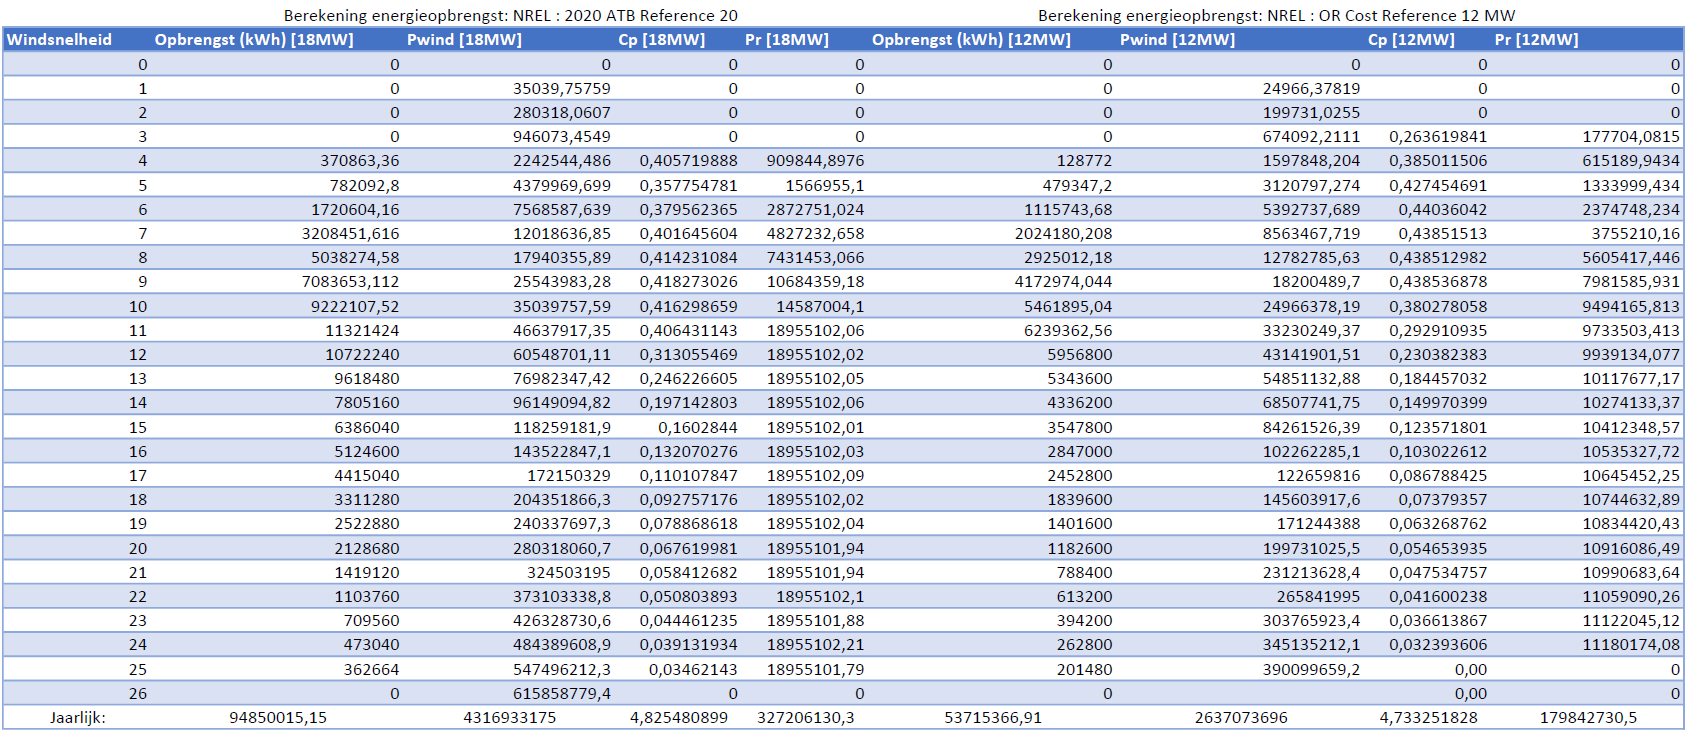
\includegraphics[width=1\textwidth]{IMG/data/overzicht/TVUW.PNG}
\caption{Gegevens: windsnelheid, energieopbrengst, vermogen en Cp}
\label{fig:TVUW}
\end{figure}

\subsubsection{Cp}
Elke windturbine heeft een vermogensfactor (Cp). Door het windvermogen te vermenigvuldigen met de Cp van de windturbine, wordt het werkelijk op te wekken vermogen verkregen. Ook de Cp is variabel, wat betekent dat het vermogen dat de turbine uit de wind kan halen ook zal verschillen afhankelijk van de windsnelheid. De plot van de Cp is te zien in (figuur \ref{fig:CpGraph}). De uitkomsten van de formules \ref{eq:5} en \ref{eq:6} zijn wederom genoteerd en geplot zoals te zien in (figuur \ref{fig:PrGraph}). 
\begin{figure}[H]
\centering
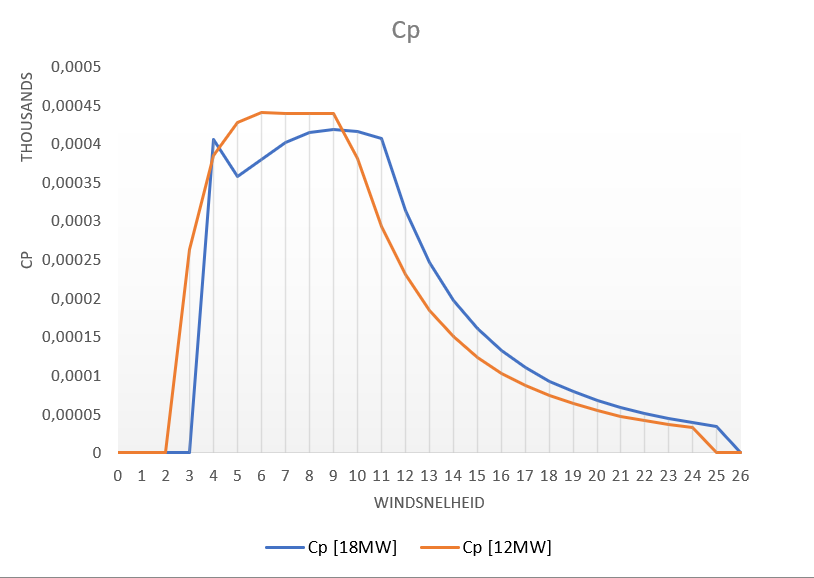
\includegraphics[width=0.7\textwidth]{IMG/data/overzicht/Cp_graph.PNG}
\caption{Plot: Cp\textsubscript{18MW} en Cp\textsubscript{12MW}}
\label{fig:CpGraph}
\end{figure}
\subsubsection{Pr}
\begin{figure}[H]
\centering
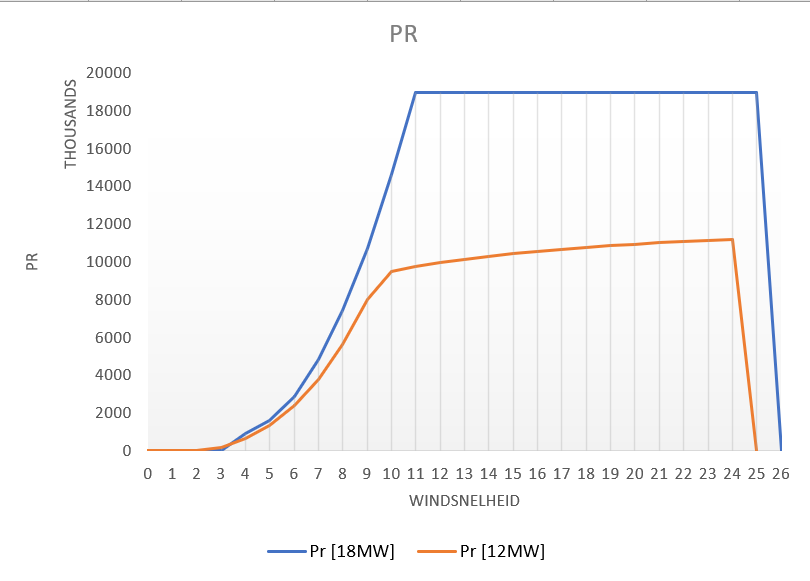
\includegraphics[width=0.7\textwidth]{IMG/data/overzicht/Pr_graph.PNG}
\caption{Plot: Pr\textsubscript{18MW} en Pr\textsubscript{12MW}}
\label{fig:PrGraph}
\end{figure}


\begin{equation} \label{eq:5}
\text{Werkelijk vermogen 12MW turbine: } P_{r12MW}=Cp_{12MW}*P_{wind12MW}
\end{equation}
\myequations{Berekening: Werkelijk vermogen 12MW turbine}

\begin{equation} \label{eq:6}
\text{Werkelijk vermogen 18MW turbine: } P_{r18MW}=Cp_{18MW}*P_{wind18MW}
\end{equation}
\myequations{Berekening: Werkelijk vermogen 18MW turbine}

\subsubsection{Wind data}
Uit de Wind Resource Assessment\cite{WindResourceAssessment} is de benodigde winddata gehaald. Hieronder valt ook informatie over de frequentie van gemeten windsnelheden gedurende een periode van twee jaar. Deze frequentie kan gebruikt worden als de kans op de windsnelheid. Met formule \ref{eq:7} kan berekend worden hoeveel uur een windsnelheid per jaar zal plaatsvinden als deze overeen komt met de bepaalde kans. In onderstaande formule (\ref{eq:7}) staat X voor de kans / het percentage dat de windsnelheid voorkomt in een jaar. 

\begin{equation} \label{eq:7}
\text{Frequentie windsnelheid in uren/jaar: } 365*24*X 
\end{equation}
\myequations{Berekening: Frequentie windsnelheid}


De verdeling van de frequentie van de windsnelheden over de span van de gemeten periode\cite{WindResourceAssessment} staat in (figuur \ref{fig:Frequentieverdeling}). 
\begin{figure}[H]
\centering
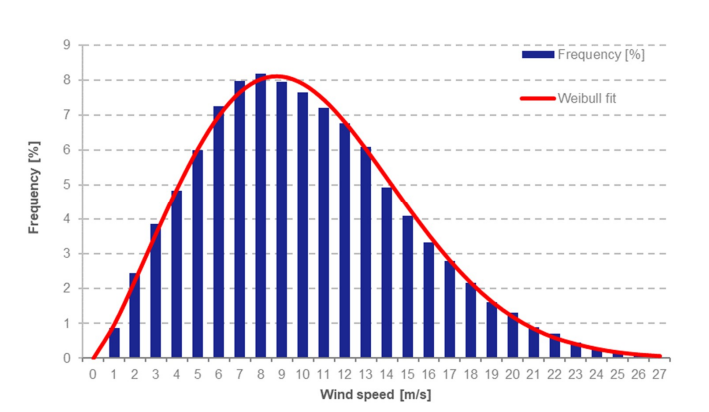
\includegraphics[width=0.7\textwidth]{IMG/data/overzicht/Frequentieverdelingwind.PNG}
\caption{Gegevens: frequentie wind snelheid per jaar.}
\label{fig:Frequentieverdeling}
\end{figure}

\subsubsection{Energieopbrengst exclusief parkeffect}
Door de verdeling van het aantal uur dat de windsnelheden voorkomen in een jaar en de berekende werkelijke vermogens van de windturbines te gebruiken, kan de jaarlijkse energieopbrengst worden berekend. Dit wordt gedaan met de volgende formules: 

\begin{equation} \label{eq:8}
\text{12MW Turbine: } E_{opbrengst,12MW}=t_{uren per jaar}*P_{r12MW}
\end{equation}
\myequations{Berekening: Energie Opbrengst 12MW Turbine}

\begin{equation} \label{eq:9}
\text{18MW Turbine: } E_{opbrengst,18MW}=t_{uren per jaar}*P_{r18MW}
\end{equation}
\myequations{Berekening: Energie Opbrengst 18MW Turbine}

De uitkomsten hiervan zijn in (tabel \ref{fig:Jaaropbrengst}) genoteerd. Nu kan de jaaropbrengst berekend worden voor beide turbines, door de uitkomsten van dezelfde turbine bij elkaar op te tellen. Hieruit is gekomen dat de jaaropbrengst met de 18MW turbine overeen komt met 94.850.015 kWh, en met de 12MW turbine overeen komt met 53.715.367 kWh. Dit verschil is behoorlijk en geeft duidelijk aan hoezo de 18MW windturbine veel voordeliger en aantrekkelijker is om te gebruiken. 
\begin{figure}[H]
\centering
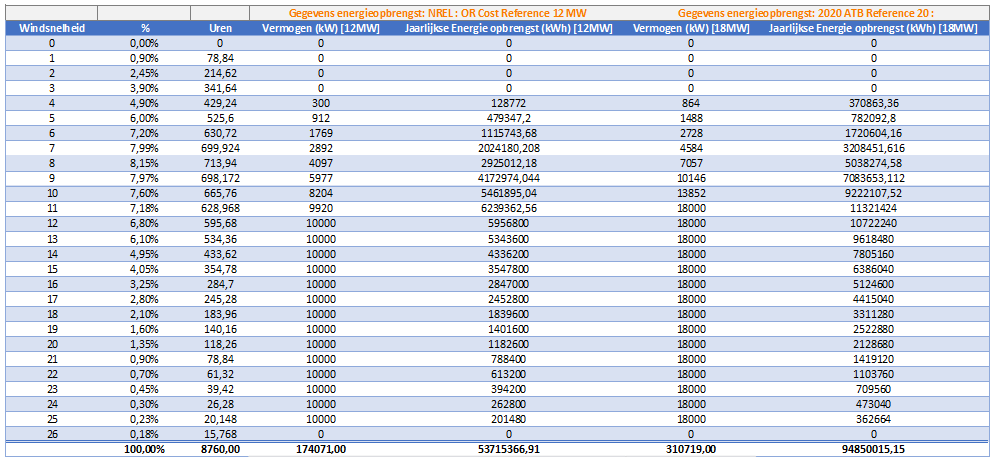
\includegraphics[width=1\textwidth]{IMG/data/overzicht/Jaaropbrengst.PNG}
\caption{Gegevens: Uren, Vermogens en Energieopbrengst.}
\label{fig:Jaaropbrengst}
\end{figure}
Bij deze jaarlijkse energieopbrengst is echter nog geen rekening gehouden met een aantal factoren die in de werkelijkheid een rol spelen, zoals het parkeffect. Om de jaarlijkse energieopbrengst inclusief het parkeffect te bepalen moet eerst het parkeffect berekend worden. Het parkeffect kan vervolgens vermenigvuldigd worden met de jaarlijkse energieopbrengst exclusief parkeffect, om de daadwerkelijke jaarlijkse energieopbrengst te krijgen. 

\subsubsection{Parkeffect}
Om dit parkeffect te berekenen, zijn een aantal tussenstappen gemaakt, waarbij verschillende berekeningen gemaakt zijn. De berekeningen moeten worden uitgevoerd voor beide kavels. Er is echter nog niet genoeg informatie gevonden over de oppervlaktes van de individuele kavels. Hier zal voor het volgende tussenrapportagemoment nog meer onderzoek naar gedaan worden. Voor nu is echter de oppervlakte van beide kavels bepaald door de oppervlakte van het windpark (176km\textsuperscript{2}) te delen door twee. Hierdoor is de oppervlakte voor beide kavels op het moment dus hetzelfde (88km\textsuperscript{2}), en verschilt er dus niks tussen de kavels. 

Om het parkeffect te berekenen zijn de volgende gegevens van belang: 
\begin{itemize}
    \item Aantal turbines per kavel
    \item Totale vermogen per kavel
    \item Oppervlakte kavel
    \item Vermogensdichtheid 
    \item Jaaropbrengst exclusief parkeffect
\end{itemize}

Ter vergelijking zijn deze berekeningen uitgevoerd voor beide windturbines. 

\subsection{Configuratie 1 (18MW)}
De eerste stap is het bepalen van het aantal turbines op de kavel. Volgens de eisen mag het totale rotoroppervlak niet groter zijn dan 2.624.613m\textsuperscript{2}, vanwege de grootte van het rotoroppervlak van de 18MW turbine, is de maximale hoeveelheid turbines die geplaatst kan worden volgens de eisen gelijk aan 48. 

De tweede stap is het totale vermogen op de kavel bepalen. Dit is het aantal turbines maal het vermogen per turbine, dus 48*18 = 864MW. Vervolgens moet de oppervlakte van het windpark bepaald worden. Hiervoor is, zoals eerder vermeld, dezelfde waarde genomen voor beide kavels, namelijk 88km\textsuperscript{2} wateroppervlak. 

Stap drie is het bepalen van de vermogensdichtheid. Om dit te berekenen kan de volgende formule gebruikt worden: 
\begin{equation} \label{eq:10}
\text{18MW Turbine: } P_{dichtheid18MW}=(\frac{n_{turbines}*P_{turbine}}{A_{oppervlak}}) = (\frac{48*18}{88}) = 9,818 MW/km\textsuperscript{2}
\end{equation}
\myequations{Berekening: P Dichtheid 18MW Turbine}

Vervolgens kan met de vermogensdichtheid het parkeffect berekend worden. Dit wordt gedaan met formule \ref{eq:11}. 

\begin{equation} \label{eq:11}
 Parkeffect_{18MW}=\frac{100-(\frac{n_{turbines}*P_{turbine}}{A})}{100} = \frac{100-P_{totaal}}{100}
\end{equation}
\myequations{Berekening: Parkeffect 18MW Turbine}

Het parkeffect varieert afhankelijk van de vermogensdichtheid. Deze is op zijn beurt weer afhankelijk van meerdere factoren. De berekende waardes van het parkeffect voor verschillende aantallen turbines staan in figuur \ref{fig:Parkeffect_table} is geplot in (figuur \ref{fig:ParkEffectGraph}). 

\begin{figure}[H]
\centering
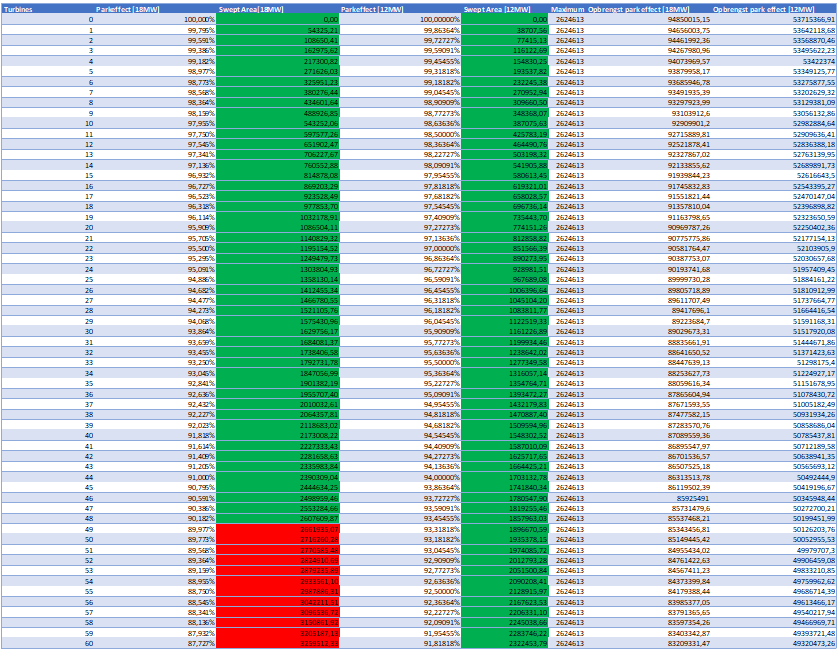
\includegraphics[width=1\textwidth]{IMG/data/overzicht/Parkeffect.PNG}
\caption{Gegevens: Aantal turbines, Parkeffect, Swept Area en Opbrengst park effect.}
\label{fig:Parkeffect_table}
\end{figure}

\begin{figure}[H]
\centering
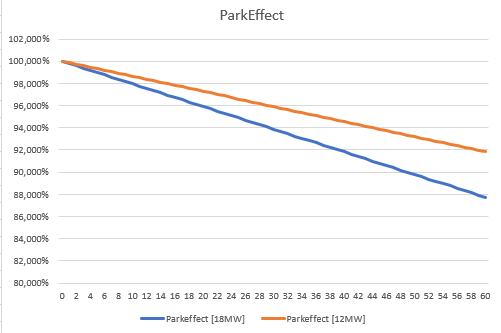
\includegraphics[width=0.7\textwidth]{IMG/data/overzicht/parkeffect_graph.PNG}
\caption{Plot: Parkeffect.}
\label{fig:ParkEffectGraph}
\end{figure}

Ten slotte kan met het parkeffect het daadwerklijke vermogen bepaald worden. Dit kan berekend worden door het parkeffect te berekenen voor het aantal turbines dat op de kavel komt. In dit geval gaat het om 48 turbines. Dus is het parkeffect: 

\begin{equation} \label{eq:12}
 Parkeffect_{18MW} = \frac{100-(P_{totaal}/A)}{100} = \frac{100-(864/88)}{100} = 0,902 = 90,2\%
\end{equation}
\myequations{Berekening: Parkeffect 18MW Turbine doorgerekend}

De jaarlijkse energieopbrengst inclusief het parkeffect is dan vrij simpel te berekenen met de formule: 
% \begin{equation} \label{eq:6}
% \text{Opbrengst 12MW kWh } t_{uren per jaar}*VermogenPerWindsnelheid_{12MW}
% \end{equation}
% \begin{equation} \label{eq:7}
% \text{Opbrengst 18MW kWh } t_{uren per jaar}*VermogenPerWindsnelheid_{18MW}
% \end{equation}


\begin{equation} \label{13}
\text{18MW Turbine: } OpbrengstParkeffect_{18MW}=Parkeffect_{18MW}*E_{opbrengst,18MW} 
\end{equation}
\myequations{Berekening: Opbrengst Parkeffect 18MW Turbine}

\begin{equation} \label{14}
OpbrengstParkeffect_{18MW}=0,902*94850015 = 85.554.713kWh 
\end{equation}
\myequations{Berekening: Opbrengst Parkeffect 18MW Turbine}

\subsection{Configuratie 2 (12MW)}
Voor configuratie 2 zijn de meeste berekeningen al uitgevoerd bij configuratie 1. Ook is het verschil duidelijk te zien in de figuren en is voor elke formule het alternatief gegeven voor de turbine van configuratie 2. 

De energieopbrengst inclusief parkeffect zal hieronder worden berekend voor de windturbine van 12MW. 

\begin{equation} \label{eq:15}
 Parkeffect_{12MW} = \frac{100-(P_{totaal}/A)}{100} = \frac{100-((60*12)/88)}{100} = 0,918 = 91,8\%
\end{equation}
\myequations{Berekening: Parkeffect 12MW Turbine doorgerekend}

\begin{equation} \label{eq:16}
OpbrengstParkeffect_{12MW}=Parkeffect_{12MW}*E_{opbrengst,12MW}
\end{equation}
\myequations{Berekening: Opbrengst Parkeffect 12MW Turbine}

\begin{equation} \label{eq:17}
OpbrengstParkeffect_{12MW}= 0,918*53715367 = 49.320.473 kWh
\end{equation}
\myequations{Berekening: Opbrengst Parkeffect 12MW Turbine}

Het verschil in jaarlijkse energieopbrengst, inclusief parkeffect, tussen de twee configuraties is dus 85.554.713 - 49.320.473 = 36.234.240 kWh aan energie per jaar. Dat is een zeer aanzienlijk getal. Dit is ook terug te zien in figuur \ref{fig:OpbrengstPark}

\begin{figure}[H]
\centering
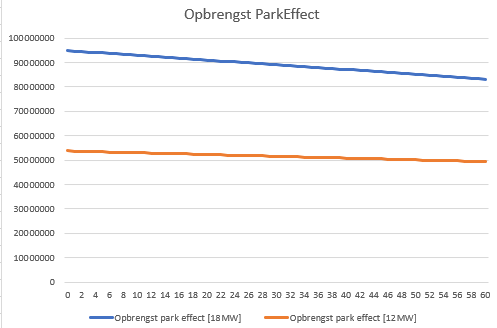
\includegraphics[width=0.7\textwidth]{IMG/data/overzicht/OpbrengstPark_graph.PNG}
\caption{Plot: OpbrengstPark.}
\label{fig:OpbrengstPark}
\end{figure}
